\documentclass[tikz]{standalone}

\usepackage{tikz}
\usetikzlibrary{decorations.pathreplacing}
\usetikzlibrary{positioning}\usepackage{etoolbox}

\begin{document}

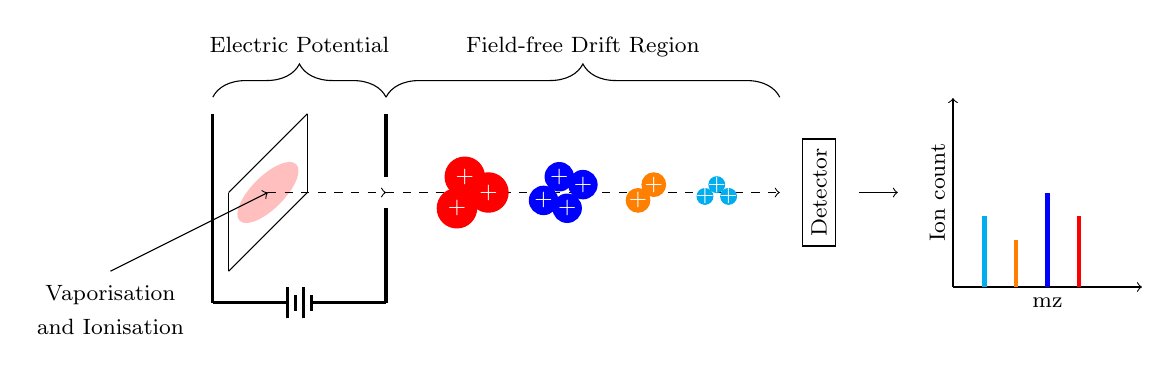
\begin{tikzpicture}
	
	\draw (0,1) -- (0,2);
	\draw (1,2) -- (1,3);
	\draw (0,1) -- (1,2);
	\draw (0,2) -- (1,3);
	\draw [fill = pink, draw = pink](0.5,2) circle [x radius = 5mm, y radius = 2mm, rotate = 45];

	\draw [<-] (0.5,2) -- (-1.5,1);
	\draw (-1.5,0.7) node {\footnotesize Vaporisation};
	\draw (-1.5,0.3) node {\footnotesize and Ionisation};
		
	\draw [very thick] (-0.2,0.6) -- (-0.2,3);
	\draw [very thick] (2,0.6) -- (2,1.8);
	\draw [very thick] (2,2.2) -- (2,3);
	
	\draw [very thick] (-0.2,0.6) -- (0.75,0.6);
	\draw [very thick] (1.05,0.6) -- (2,0.6);
	
	\draw [very thick] (0.75,0.4) -- (0.75,0.8);
	\draw [very thick] (0.85,0.5) -- (0.85,0.7);
	\draw [very thick] (0.95,0.4) -- (.95,0.8);
	\draw [very thick] (1.05,0.5) -- (1.05,0.7);
		
	\draw [decorate,decoration={brace,amplitude=12pt},yshift=6pt]
					(-0.2,3) -- (2,3) node [black,midway,yshift=19pt] 
{\footnotesize Electric Potential};
	
	\draw [->,dashed] (0.5,2) -- (2,2);
	\draw [->,dashed] (2,2) -- (7,2);
	
	\draw [fill = red, draw = red] (3.3,2) circle [radius = 2.5mm];	
	\draw (3.3,2) node {{\footnotesize{\color{white} $+$}}};
	\draw [fill = red, draw = red] (3.0,2.2) circle [radius = 2.5mm];	
	\draw (3.0,2.2) node {{\footnotesize{\color{white} $+$}}};
	\draw [fill = red, draw = red] (2.9,1.8) circle [radius = 2.5mm];	
	\draw (2.9,1.8) node {{\footnotesize{\color{white} $+$}}};
	
	\draw [fill = blue, draw = blue] (4.5,2.1) circle [radius = 1.8mm];	
	\draw (4.5,2.1) node {{\footnotesize{\color{white} $+$}}};
	\draw [fill = blue, draw = blue] (4.3,1.8) circle [radius = 1.8mm];	
	\draw (4.3,1.8) node {{\footnotesize{\color{white} $+$}}};
	\draw [fill = blue, draw = blue] (4.0,1.9) circle [radius = 1.8mm];	
	\draw (4.0,1.9) node {{\footnotesize{\color{white} $+$}}};
	\draw [fill = blue, draw = blue] (4.2,2.2) circle [radius = 1.8mm];	
	\draw (4.2,2.2) node {{\footnotesize{\color{white} $+$}}};
	
	\draw [fill = orange, draw = orange] (5.2,1.9) circle [radius = 1.5mm];	
	\draw (5.2,1.9) node {{\footnotesize{\color{white} $+$}}};
	\draw [fill = orange, draw = orange] (5.4,2.1) circle [radius = 1.5mm];	
	\draw (5.4,2.1) node {{\footnotesize{\color{white} $+$}}};
	
	\draw [fill = cyan, draw = cyan] (6.2,2.1) circle [radius = 1mm];	
	\draw (6.2,2.1) node {{\footnotesize{\color{white} $+$}}};
	\draw [fill = cyan, draw = cyan] (6.05,1.95) circle [radius = 1mm];	
	\draw (6.05,1.95) node {{\footnotesize{\color{white} $+$}}};
	\draw [fill = cyan, draw = cyan] (6.35,1.95) circle [radius = 1mm];	
	\draw (6.35,1.95) node {{\footnotesize{\color{white} $+$}}};
	
	
	
	\draw [decorate,decoration={brace,amplitude=12pt},yshift=6pt]
					(2,3) -- (7,3) node [black,midway,yshift=18pt] 
{\footnotesize Field-free Drift Region};




	\node [draw, rotate=90] at (7.5,2) {\footnotesize Detector};
	
	\draw [->] (8,2) -- (8.5,2);

	\node [draw = none, rotate=90] at (9,2) {{\footnotesize Ion count}};	
	\draw [->] (9.2,0.8) -- (9.2,3.2);
	\draw (10.4,0.6) node {{\footnotesize \gls{mz} }};
	\draw [->] (9.2,0.8) -- (11.6,0.8);
	
	\draw [draw = cyan, ultra thick] (9.6,0.8) -- (9.6,1.7);
	\draw [draw = orange, ultra thick] (10,0.8) -- (10,1.4);
	\draw [draw = blue, ultra thick] (10.4,0.8) -- (10.4,2);
	\draw [draw = red, ultra thick] (10.8,0.8) -- (10.8,1.7);
	
	
	
	
\end{tikzpicture}

\end{document}